\chapter{Implementation}



This chapter focuses on practical implementation with respect to the Domain Legitimacy Checker. The multi-viewed approach, along with programming in Python and the web framework in Flask, HTML, CSS, JavaScript, on the side of external APIs, assisted greatly in making a resilient framework for DNS abuse detection and transparency improvement. With those alternatives, I came up with this simple but effective way of not just finding legitimacy in domain names but also of showing plainly and clearly the various tactics with which bad actors are using in the adoption of confusable domains for phishing and malware distribution, along with other malicious activities to help me with my research. This endeavour embarked on a journey from the idea to execution, focusing on a user-friendly web interface that allows users to quickly identify potentially malicious domains. 

\section{System Overview}

Domain Legitimacy Checker is such a robust web-based platform tasked with the identification and analysis of domain names that can be malicious. The user first initiates the domain name requests through the user interface. This request is processed by the Flask-based web server orchestrating the core operations of the system. Domain Analysis Engine is meant to perform an analysis on DNS abuse patterns exhibited by the submitted domain using heuristics and pattern matching algorithms. For a deep check, the system queries external APIs such as VirusTotal for additional checks of legitimacy. The results of such checking are kept in a Database as well, which gives out the history of known malicious domains. Finally, the Results Display component gives control of the results back to the user. Figure \ref{fig:figfig} provides an illustrative view of the architecture of design of the software system and the information flow.


\begin{figure}[H]
\captionsetup{font= footnotesize}
    \centering
    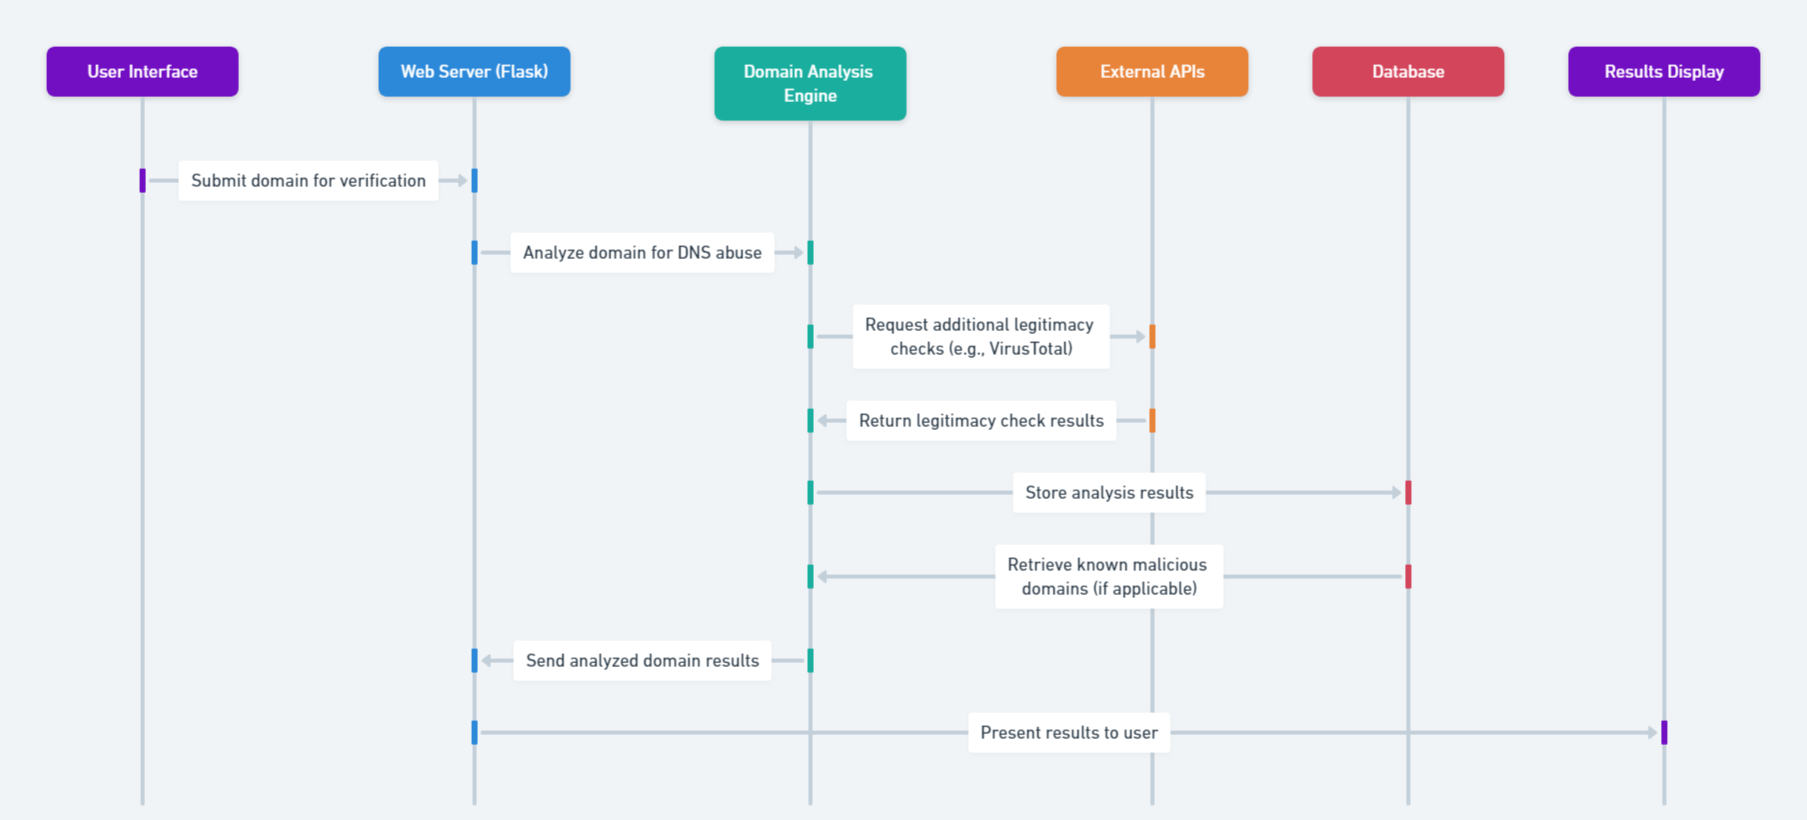
\includegraphics[width=1\linewidth]{project/DNS Abuse Transparency System.png}
    \caption{Domain Legitimacy Checker}
    \label{fig:figfig}
\end{figure}

\section{Integration} 
\subsection{Backend Implementation}

The server side :  Python on the Flask framework was used for implementing this side. The server works better with a solid web server in case you are time pressed because the learning curve on Flask to make it implement is not that steep. The Flask application is set to work through a series of endpoints, each of which corresponds to a set of functionalities with respect to the system, among which is an endpoint for submitting domains to ascertain the results of their analysis. A request comes into the Flask server, and for any incoming given request, it simply calls the indicated function to handle the process relevant to the request: a process to parse the input data, to start domain checks, or to respond with the check results.

 API \& library : The Domain Analysis Engine forms the main core within the backend, responsible for DNS abuse detection. This is realised by creating some of the changes that the submitted forms of domain names have so that possibly malicious or confusable counterparts are recognised with the assistance of pattern recognition algorithms. In addition, the development leverages libraries and packages such as "dnspython" and requests to conduct the queries to DNS and "request" APIs with respective libraries. This system communicates with external APIs such as "VirusTotal" in order to perform legitimacy checks, whereby the fact is made up for carrying out thorough analysis and reliable detection of malicious domains.

 \begin{figure}[H]
     \centering
     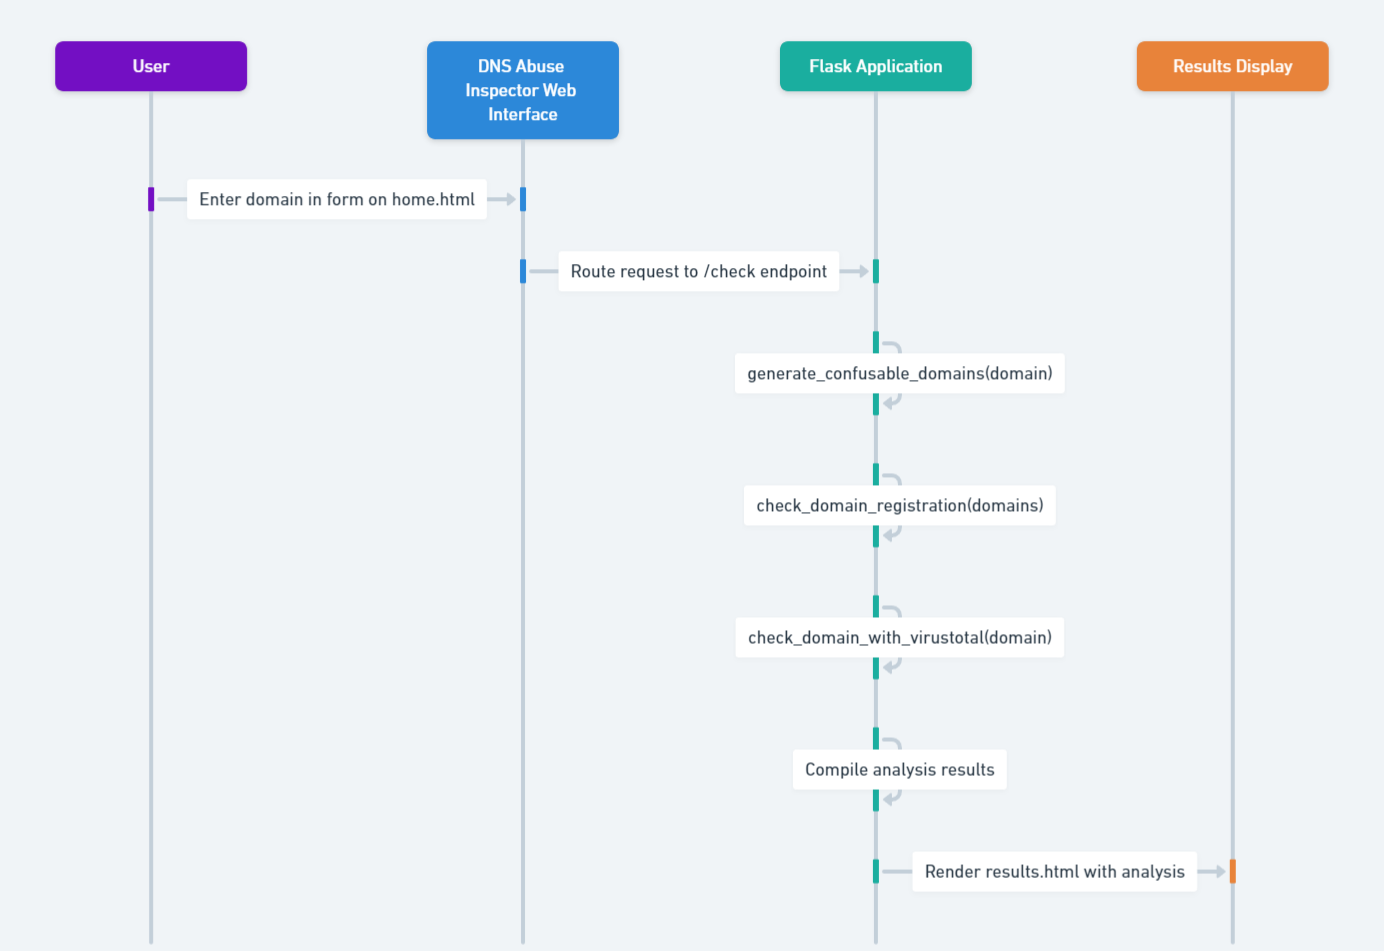
\includegraphics[width=1\linewidth]{project/Domain Legitimacy Check Workflow.png}
     \caption{Domain Legitimacy Checker System Interaction Workflow}
     \label{fig:figfigfig}
 \end{figure}

\subsection{Frontend Implementation}

Web Interface: HTML was used and then styled with CSS, and fine-tuned with Bootstrap, the user interface has responsiveness built in and is very user-friendly for use, regardless of the device that it is being used on. The interface is user-friendly, from submission of the initial domains easily, to displaying results, intending an automatically flowing process designed simple to the layman.


Interactive elements: JavaScript is used to bring in interactivity to most of the pages, mostly through the main.js file, bringing the most important interactivity to the web app domain submission pages. These respects real-time, giving feedback even for the submission of domains, for instance, changing the text of the submission button to "Analysing." and avoiding its swarming with submissions. These dynamic elements in the front-end make the process of domain analysis even more visually responsive, which increases users' engagements and trust in how the system processes.

\begin{figure}[H]
    \centering
    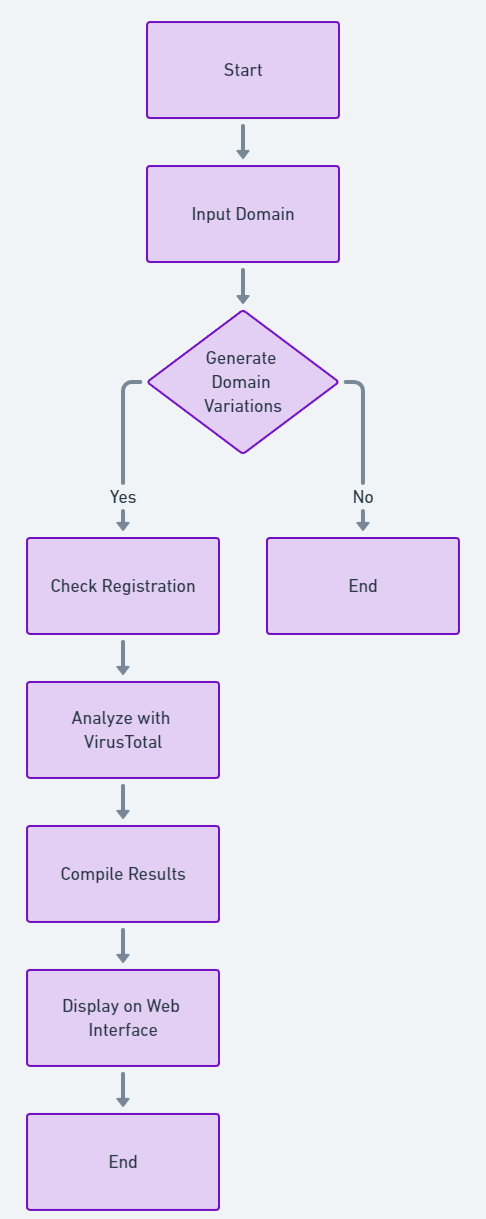
\includegraphics[width=0.6\linewidth]{project/DNS Abuse Inspector Operational Flowchart.png}
    \caption{Domain Legitimacy Checker}
    \label{fig:figfigfig}
\end{figure}
\newpage


\section{Tools \& Technologies}

The Domain Legitimacy Checker was built using a carefully selected stack of tools, languages, and platforms. The primary language chosen was Python, valued for its readability, comprehensive standard library, and wide range of third-party modules that facilitate rapid development and integration with other systems. As a result, the decision was made to stick with Flask as an interactive back-end web framework, since, in connection with its extremely light character, it is easily scalable in nature. Though designed very simple, it's versatile enough to really cover all major issues regarding painful threads of HTTP-requests processing. For the front-end, HTML5 was the markup language of choice to structure content on the Web, while CSS3 was used for styling, to ensure a modern and engaging user interface. Bootstrap, a widely used front-end framework, was integrated to accelerate responsive design, allowing the interface to adapt to various device screens without extensive custom code. It is very important to ensure that a system runs smoothly by making the development of dynamic and interactive web pages using JavaScript. In the system, the scripting at the client side has used plain JavaScript so that it may maintain simplicity and hold onto any control over all the behaviours implicated.The dnspython library provided the tools necessary for DNS queries, allowing the system to interact with DNS records, an essential feature for checking domain registration status. To conduct external checks for domain legitimacy, the requests library facilitated communication with external APIs, such as VirusTotal, renowned for its extensive database and reliable threat analysis. 

The VirusTotal API was used because of its comprehensive scanning capabilities, which leverage a multitude of antivirus engines and website scanners to assess the security of a domain. The scope of its scanning will come from thousands of antivirus engines and websites that will check if the domain is safe to browse or download. Equally important in the system is the ability to establish the analysis of a wide spectrum of potentially abusive domains. VirusTotal searches for a record of whether the supplied domain has ever been blacklisted before for hosting phishing sites, spreading malicious software, or, in general, being accessed for carrying out other suspicious actions. Such a dataset is to be found within the very repository of the API, thereby making available unmatched data and accuracy for threat detection, hence by and large enhancing the capability of this system in terms of protection against DNS related cyber threats.


Each tool and technology were chosen not only for its individual merits, but also for how well it integrated with the others, ensuring a cohesive and efficient system aligned with the project's objectives of DNS abuse detection and transparency.

\section{Visualisations}

The interface and layout of the web page have been designed for ease and smooth transition with users. It was specially designed the interface through which our users can easily verify if the domain is legitimate. As with all its applications. Upon loading, the Domain Legitimacy Checker presents itself within a very neat and simple layout. The hero section comes with the name of the application. The domain name input field is at the heart of the page, which requires the user to type the domain url they wish to analyse. Once a domain is submitted, the system spring into action, processing the input through various checks and analyses. The server logs these interactions, as seen in subsequent visualisations, ensuring that every step of the process is recorded for performance monitoring and optimisation.

\begin{figure}[H]
    \centering
    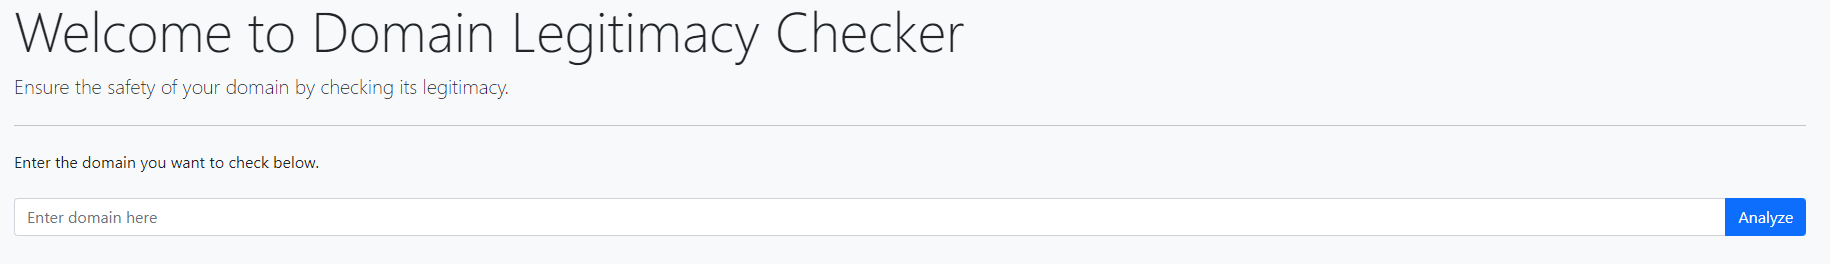
\includegraphics[width=1.1\linewidth]{project/image.png}
    \caption{The main interface of the Domain Legitimacy Checker}
    \label{fig:implem22}
\end{figure}

\subsection{Input \& Interaction}

 The Domain Legitimacy Checker Tool provides an intuitive and streamlined place for interaction with users to ensure a seamless experience.The domain input method, a single-field form intended for simplicity of use and quick analysis, is at the centre of this interaction.
 
\begin{figure} [H]
    \centering
    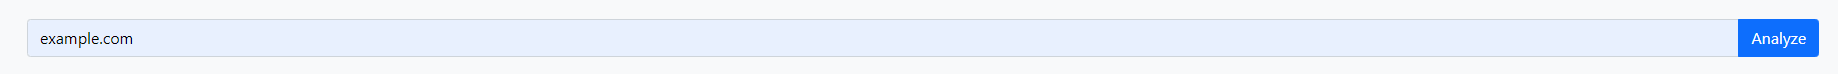
\includegraphics[width=1.1\linewidth]{project/6.png}
    \caption{The domain input box where users begin their interaction with the Domain Legitimacy Checker.}
    \label{fig:impl2}
\end{figure}

First, the user is asked to enter a domain of their choice and to put it in a text box, minimally styled to not distract but to point the user's focus in performing the task. Right next to the text box is the "Analyze" button, contrasting with blue to stand out visually and identified for the user as the next step to take in the process. This design invites immediate action upon domain entry, providing a clear path from user input to results.

\begin{figure}[H]
    \centering
    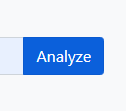
\includegraphics[width=0.3\linewidth]{project/8.png}
    \caption{The 'Analyze' button, poised for user action after domain entry.}
    \label{fig:imple2222}
\end{figure}

The user's request to check a domain is initiated as soon as a domain is entered into the 'Analyze' field and the button is hit: a series of background checks are run to understand the eligibility of the domain. It is at this point with the changing request of the user that his request is no longer an action but a graph analysis that is being done by the systems running in the back end.

\subsection{Interactive Features}

The program comes with an interactive interface; the user is engaged at all steps from entering a domain for analysis right down to receiving the results. In fact, starting from the second users have done submitting a domain for analysis, this very step will start a circle of HTTP-requests, which the server logs with great care. These logs are dynamic, real-time visualisations of user-server interaction rather than just recordings.


The moment a 'click' on the 'Analyze' button happens, the server instantly receives a 'POST' request through the endpoint '/check', which notes that the action marks the start of the domain analysis. On a successful request, a '200' status cookie is returned to signify a successful search. Such type of interactions goes down as entries into the server log, forming a very critical and highly detailed timeline of activities.
\begin{figure}[H]
    \centering
    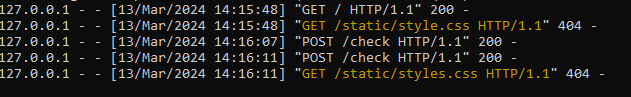
\includegraphics[width=0.8\linewidth]{project/I.png}
    \caption{Server log entries capturing real-time HTTP requests and responses}
    \label{fig:imple22222}
\end{figure}

If there is any issue, these logs are highly important for example, in the case of "404 - Not Found" error in the requested resource. They do not only instantly inform what might have gone wrong to system administrators, but also act as hints for such troubleshooting. Log analysis allows an administrator to automatically correct problems.

\subsection{Results Display}

The Domain Legitimacy Checker displays the findings in an easy-to-understand style after the completion of the domain legitimacy research. Every domain has an icon next to it; a  exclamation point indicates that the domain is possibly harmful, and a  check-mark indicates that the domain is not malicious. The initial level of result interpretation is this instantaneous visual feedback, which enables users to assess domain safety rapidly.

\begin{figure}[H]
  \centering
  \begin{subfigure}[b]{0.45\textwidth}
    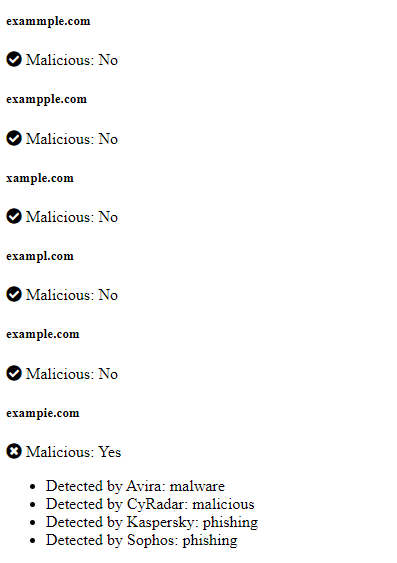
\includegraphics[width=\textwidth]{project/inhg.png}
    \label{fig:left}
  \end{subfigure}
  \hfill % adds horizontal space between the figures
  \begin{subfigure}[b]{0.45\textwidth}
    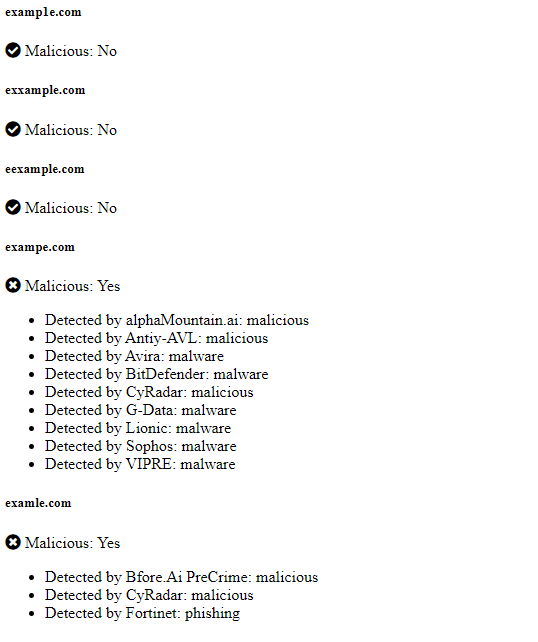
\includegraphics[width=\textwidth]{project/oooo.png}
    \label{fig:right}
  \end{subfigure}
  \caption{visual indicators showing the legitimacy status of analysed domains.}
  \label{fig:images}
\end{figure}

For domains identified as malicious, the interface unfolds additional information, providing a breakdown of the detected security threats. Each scanner's findings are listed beneath the domain, revealing the specific categories of malicious activity identified, such as malware, phishing, or other security threats. This level of detail is not only informative but also actionable, guiding users on potential next steps for mitigation or further investigation.

\subsection{Navigating Results}

After the results from the domain check come back, the Domain Legitimacy Checker would then allow the user to easily explore more domains that interest them. It normally does this through a button that shows prominently on the interface for this function and which simply says "Check Another Domain." Basically, this re-engages the user with the input interface.

\begin{figure}[H]
    \centering
    
\includegraphics[width=0.3\linewidth]{project/ii.png}
    \caption{The 'Check Another Domain' button}
    \label{fig:enter-label}
\end{figure}

This iterative process is another valuable characteristic of the user journey, so it can be continued non-stop right on the search results page. This squarely builds on the design philosophy of the tool, that of making the user capable of doing as many searches in as lean a manner as possible, fostering an environment of proactive web security.




\section{Challenges \& Solutions}

During the development of the Domain Legitimacy Checker, I faced several challenges, each requiring a tailored solution to ensure the project's success.

Challenge 1: API rate limit
The frequent use of the VirusTotal API presented a challenge due to its rate-limiting constraints. Exceeding the allotted number of requests would lead to temporary blocking of our service.

Solution: Implementing a queuing system with a delay mechanism to spread the requests over time, adhering to the API's rate limits. Additionally, we cached the results of previous queries to minimise repeat requests for the same domains.

Challenge 2: Real-time Feedback for Users, therefore, is very important to give very instant feedback in the process of the domain analysis, but was otherwise very hard to prove because of the asynchronous behaviour, in principle for network operations.

Solution: Using asynchronous JavaScript to send information to the servers and receive results from them without refreshing the web page. 

Challenge 3: Handling Malicious Domain Variations
Identification and generation of a full set of confusing domain variations represented a key computational challenge.

Solution: Using a combination of common substitution algorithms and a heuristic approach that prioritised variations based on their likelihood of being used in phishing attacks. 

Challenge 4: Data Storage \& Retrieval Efficiency
Storing analysis results for quick retrieval while managing database performance was a concern, especially with the growth of the data set.

Solution: implementing a real-time domain analysis system with external APIs for comprehensive domain validity checks and algorithmic domain variation creation to assess potential security risks. 
 
Challenge 5: System Scalability
As the system's user base grows, so does the load on our servers, which initially led to concerns about scalability.

Solution: The system was designed with scalability in mind, using Flask's built-in capabilities to handle an increasing number of simultaneous user requests. 

By addressing these challenges with careful planning and adaptive solutions, we improve the reliability, performance, and user satisfaction of the system.

\section{Testing \& Validation}

The Domain legitimacy checker follows rigorous measures in testing the system, which ensures both dependability and accuracy. In the implementation, the back-end logic had a number of things implemented with unit tests; we have used the Python unittest framework. We used mock objects to simulate the acts of external APIs.Manual and automated tests were performed in front-end technologies. Automated UI testings, such as those with Selenium, were relied upon to ensure that all interactive elements are operable. The interface has been tested both automatically and manually, with the help of loading a page on a few browsers and mobile devices to ensure that the interface is responsive and behaves similarly. Continuous Integration (CI) pipelines was set up so that every time a new code commit passes to run tests, ensuring that newly made changes do not break existing functionalities automatically. 

